\documentclass[12pt,twoside]{article}

\usepackage{amsmath}
\usepackage{fancyhdr}
\usepackage{graphicx}

\setlength{\oddsidemargin}{0pt}
\setlength{\evensidemargin}{0pt}
\setlength{\textwidth}{6.5in}
\setlength{\topmargin}{0in}
\setlength{\textheight}{8.5in}
\setlength{\headheight}{15pt}

\newcommand{\andrew}{Andrew Xia}
\newcommand{\psetnum}{6.115 Final Project Proposal Draft}
\newcommand{\duedate}{Due: April $5^{\text{th}}$, 2016}
\renewcommand{\thesubsection}{\thesection.\alph{subsection}}

\pagestyle{fancy}
\fancyhead[L]{\andrew}
\fancyhead[C]{\psetnum}
\fancyhead[R]{\duedate}

\begin{document} 
\begin{center} {\bf \large \psetnum}
\\ \emph{Hardware Implementation of Tinder}
\\ {\bf \andrew}
\\ \duedate
\end{center}

\section{Introduction}
It's Spring 2016, and we're here with another spectacular 6.115 project proposal! In this project, I propose to integrate two key parts of a 6.115 student's life, to create my final project for the Microcotrollers Project Laboratory class. By day, students spend time in the 38-600 lab to work on our lab projects. By night, we are glued to our cell phones, interacting with real and somewhat imaginary friends through social media apps. Thus, in order to capture the quintessential essence of a 6.115 student, I propose to implement, for my final project, a {\bf Hardware Version of Tinder}.
\\
\\ Tinder is a social media app that facilitates communication between mutually interested users. In this location-based app, users scan through other registered people in the application and can swipe right to show interest or swipe left otherwise. The app allows matched users to chat, and subsequent meetups are to the users' disgression. In my implementation fo Tinder, I plan to keep the spirit of the application while modifying the user interface to allow for more hardware based interactions. 
\\
\\ \emph{What interested you in the idea?} When thinking about my project idea, I wanted to create a final project that would both give me an opportunity to further learn how to use microcontrollers, and also make a project that would be entertaining and fun to use. Coming from a background with more software than hardware experience, I initially considered ideas on the product axis instead of the technology axis, and eventually settled upon the tinder idea. 
\\ 
\\ \emph{Why is this project interesting?} Since social media in our current day and age is a huge part of our lives, users would naturally be interested in testing out my project. With familiarity knowing the concept of my project, and also a degree of unfamiliarity in seeing a new implementation of a social media app beloved by all, I believe that my project will be very interesting and enjoyable for users. 
\\ While the app Tinder is mainly a software-based product, I believe that I can also engineer the concept into one that would involve physical hardware features to better the user experience. Some ideas and features that I am thinking about including are:
\begin{itemize}
\item Add a LED light based sensor to detect a user swiping right or swiping left. The LED can also be speed-based to detect how strong of a like or dislike a user wants to express
\item Use either my Amulet module or a VGA connection from the 8051 to display users profiles on a screen. 
\item In order to collect a large database of users, I can either pull data from Tinder's API online (and learn how to connect my 8051 using a router to the internet) or I could send out surveys and forms to the MIT community to populate my database. 
\item In order to log on to one's tinder account on the 8051, I could have a LED matrix board, in which users could depress buttons or cover up lights as a command input. Depending on the arrangement of the depression, the program will detect which user has logged on. 
\end{itemize}


\section{Hardware Description}

There will be two user input modules for my Hardware Implementation of Tinder. The first is a LED light-based motion sensor, in which I will have two LED lights and LED light sensors similar to the Lab 4 SpinDude set up five inches apart from each other. A low signal means that the user's hand is blocking the LED light, and based on the sequence of the two LED lights falling to low, we can determine the direction of swiping. The ADC0804 will detect whether a signal is high or not and communicate with my 8051.
\\ The second user input component is a Laser Cut board that I plan on designing for user password recognition. In order to check which user is logging into the 8051 for his or her respective Tinder Account, I plan to have a board of buttons, and the user can press a series of buttons for his keypad to form his login password sequence. The information will be sent to the 8051 via the 8255.
\\ As for the output display, I plan to use a VGA display screen powered by the PSoC to display information about the peoples' Tinder Profiles. We will connect with the PSoC over using a 8051 as it is more powerful and can provide a higher resolution and faster-updating display. 
\\ Depending on data storage needs, I may also include an extra RAM chip. 

\subsection{Hardware Schematic}
Below is a preliminary hardware schematic of my final project:
\begin{center}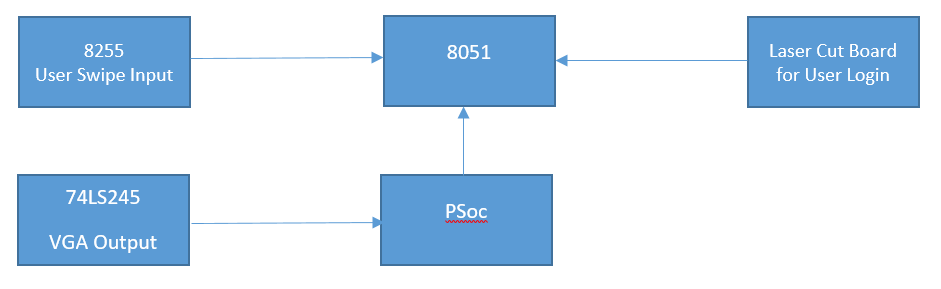
\includegraphics[width = 150mm]{Hardware.png} \end{center}

\section{Software Description}
As for my software, I will code my project in C, using the PSoC as my main control module, as it would would be more efficient to do so over writing code in assembly for the 8051. Tinder is quite software heavy, so I hope to develop the basic framework for my code and spend the rest of my extra time focusing on hardware improvements. 

\subsection{Software Flowchart}
Below is a flowchart of my software: 
\begin{center}\fbox{\begin{minipage}{30em}

\begin{enumerate}
\item User Login
\item User is presented with Person
	\begin{enumerate}
	\item User is given description of Person on VGA display
	\item User can “laser swipe right” to “like” or “laser swipe left” to “dislike”.
	\end{enumerate}
\item Algorithm for recommending next person based on matched peoples’ interests.  
\item If user is matched, contact information is given. 
\end{enumerate}

\end{minipage}} \end{center}
In step 1, the user logins into his account through entering in a password. The software will check which LED lights the user has depressed, and proceed onto the Tinder game. In step 2, the user is presented with a person on the VGA display, displaying information such as name, interests, pictures, and a funny quote from the person. The user can communicate with the game by either swiping right to show interest, or swiping left otherwise. Based on the user's swiping pattern and the similarity of the displayed people, we can also design an algorithm to recommend following people to optimize matching. If a match has been detected (in which both users have shown interest towards one another), then contact information can be given to further facilitate communication between the two. 

\section{Project Scope and Management}

\subsection{Modest risk level Project goals}
In this section, I will discuss goals for my project that I can meet with high probablity. At a very basic level, I hope to build the swipe sensing module, which would be two LED lights and two LED sensors to detect movement. I would not have the VGA connected; instead I could have text be printed in the SecureCRT terminal. My tinder software would be static, having a list of users, some predefined to be matchable, others not, and there would be no password input board.

\subsection{Adding the wow factor}
In this section, I will discuss goals for my project that I plan to meet. I want a working Tinder algorithm, that I can display on the secureCRT terminal. I will have collected a lot of user data so there will be a large pool of users available for the user to swipe to. I also want to have my VGA display working, so I can display information about people interactively on a larger display. 

\subsection{To make the project SPECTACULAR}
In this section, I will goals for my project that I will explore if I have time during the semester. I hope to have a password module working, in which users can depress a set of buttons or be scanned from a matrix of LED lights or sensors to login into their account on my microcontroller. In addition, I could consider adding additional hardware features, or software features such as a recommendation based algorithm. 


\section{Special Component Needs}
\emph{What special chips will I need?} 74LS245, VGA pin. 


\section{Timetable}
\begin{enumerate}
\item April 11-18
\\ \indent During this week, I plan to build a basic LED swipe detection module. 
\item April 18-25
\\ \indent During this week, I hope to write a basic software interface for Tinder, allowing users to swipe right and left to communicate with my software. 
\item April 25-May 2
\\ \indent During this week, I hope to set up my VGA connection and allow my software to be displayed on a larger screen.
\item May 2 - 9
\\ \indent During this week, I want to set up a password module, in which users can login into their accounts and swipe accordingly to their personal interests. 
\item May 9 - 15
\\ \indent During this week, I can further improve the software or hardware aspects of my project, such as adding a recommendation based algorithm or add further swipe interaction possibilities. 
\end{enumerate}

\end{document}